\documentclass[11pt]{article}
%\usepackage{endfloat}
\usepackage[paperwidth=8.5in,paperheight=11in,margin=1in]{geometry}
\usepackage{xr}
\externaldocument{paper}
%% HACKS %%
 
% For section headers starting with S
\renewcommand{\thesection}{S.\arabic{section}}
\renewcommand{\thesubsection}{\thesection.\arabic{subsection}}
 
% Hack for making SOM Equations Conform to Science Format
%
% e.g. (S1), (S2), etc
% Requires AMS
\makeatletter %% With ams
\def\tagform@#1{\maketag@@@{(S\ignorespaces#1\unskip\@@italiccorr)}}
\makeatother
 
% Hack for making figures Say \figurename S\thefigure, e.g. Figure S1:
%\makeatletter
%\makeatletter \renewcommand{\fnum@figure}
%{\figurename~S\thefigure}
%\makeatother
 
% use bibnumfmt to change style at the end of the document
%\renewcommand{\bibnumfmt}[1]{[S#1]}
% citenumfont command adds S to all numbers
%\newcommand{\citenumfont}[1]{\textit{S#1}}
 
\newcommand{\myfigurename}{Figure}
\newcommand{\myref}[1]{\ref{#1}}
\newcommand{\suppref}[1]{S\ref{#1}}
\newcommand{\suppfigurename}{Figure}
 
\usepackage{tikz}
\usepackage{amsmath}
\usetikzlibrary{automata, arrows, positioning, shapes, snakes}
 
%END HACKS

\usepackage{graphicx}

\title{Supporting Information}
\author{}
\begin{document}

%We want to assay every site in the genome
%Accurate whole genome sequencing is too expensive
%SNP arrays and low-pass sequencing are therefore the most used
%technologies
%They have different strengths and weaknesses
%A principled integration framework might improve calling


\maketitle

\section{Model}

For each variant, we model its phenotypic effects as shown in Figure
\myref{fig:variantbn}. We assume that the effect of the variant on a
single endophenotype ($E$) determines its effects on a number of other
traits ($T_1, T_2, \ldots, T_q$). The effect on each trait $T_i$ then
determines its measured effect on that trait $O_i$. Furthermore,
conditional on observing the true effects $T_i$ on all traits, the
observed trait effects $O_i$ are conditionally independent. Finally,
conditional on observing the effect on the endophenotype $E$, the
true effects $T_i$ are conditionally independent of each
other. Dependencies among traits not captured by $E$ could be added,
but we omit these for now.

\begin{figure}[ht]
\begin{center}
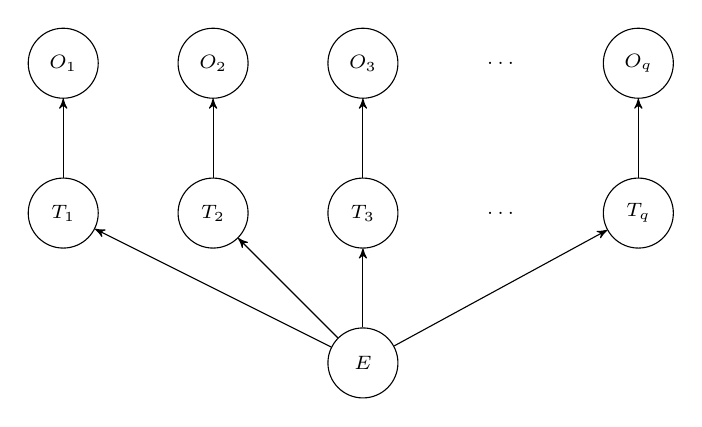
\begin{tikzpicture}[>=stealth',auto, font=\scriptsize]
  \tikzset{ellipse/.style={draw,ellipse}}

  \tikzset{
    blank/.style={
      text centered},
    circ/.style={
      circle,
      draw=black,
      minimum height=.35in,
      text centered}}

  \node[circ] (to1) {$O_1$};
  \node[circ] (to2) [right=of to1] {$O_2$};
  \node[circ] (to3) [right=of to2] {$O_3$};
  \node[blank] (tospace) [right=of to3] {$\ldots$};  
  \node[circ] (ton) [right=of tospace] {$O_q$};
  \node[circ] (t1) [below=of to1] {$T_1$};
  \node[circ] (t2) [below=of to2] {$T_2$};
  \node[circ] (t3) [below=of to3] {$T_3$};
  \node[blank] (tspace) [right=of t3] {$\ldots$};  
  \node[circ] (tn) [below=of ton] {$T_q$};
  \node[circ] (endo) [below=of t3] {$E$};

  \path[->] (endo) edge (t1);
  \path[->] (endo) edge (t2);
  \path[->] (endo) edge (t3);
  \path[->] (endo) edge (tn);

  \path[->] (t1) edge (to1);
  \path[->] (t2) edge (to2);
  \path[->] (t3) edge (to3);
  \path[->] (tn) edge (ton);

\end{tikzpicture}
\end{center}
\caption{Model for phenotypic effects of a variant}
\label{fig:variantbn}
\end{figure}

We then specify conditional probability distributions as:
\[ E \sim {\mathcal N}\left(\mu, \tau^2\right) \]
\[ T_i \sim {\mathcal N}\left(\beta_i E, \sigma_i^2\right) \]
\[ O_i \sim {\mathcal N}\left(T_i, s_i^2\right) \]

The intuition behind the parameters is as follows. The $\beta_i$ control the relative values of the effects of the
endophenotype on each of the traits, or in other words the
``phenotypic profile''. They are relative values; if a variant has a
two-fold effect on the endophenotype relative to another variant, it
will have two-fold stronger effects on each of the traits, but the
relative effects across traits will be the same between the two
variants. The $\sigma_i$ parameters control how important each trait
is in the phenotypic profile; small values will insist that variants
with the same endophenotype effects $E$ have very similar effects on
the trait, while larger values will allow variants with similar
endophenotype effects to have discrepant trait effects.

$\mu$ and $\tau$ control the prior population distribution of $E$. Many times $\mu$ will be
set to 0; however, in some cases (such as modeling variants from
within a disease gene) it may be desirable to have $\mu \neq
0$. $\tau$ controls the ``prevalence'' of the endophenotype; small values of $\tau$
will bias more variants to have small effects $E$ on the
endophenotype.

The $s_i$ values control the sampling distribution of the observed
association statistics. They will depend on the frequency of the
variant and the population in which it is tested for association.

Specification of these distribution allows us to answer several
questions. For example:

\begin{enumerate}
  \item {\bf What is the posterior distribution of effects on one
    trait $T_i$, given observed effect on other traits $O_1,\ldots,O_{i-1},O_{i+1},\ldots,O_q$?} We would run the
    query $\Pr\left(T_i \mid O_2,\ldots,O_q\right)$. The means of
    this posterior could be used for weights in an aggregate test, or
    the distributions could be used to filter variants for
    inclusion. Alternatively, this could be used as a prior in a
    Bayesian association analysis.
    \item {\bf What variants affect specified endophenotype?} For each
      variant, we would compute $\Pr\left(E\mid T_1,\ldots,T_q\right)$.
\end{enumerate}

\section*{Fitting the model}

To use this model, we need to learn the parameters $\mathbf{\theta} = \mu, \tau,
\beta_i, \sigma_i,$ and $s_i$.

For $s_i$, we assume that the variance
of the observed coefficient $O_i$ is equivalent under the null distribution
($T_i = 0$) and the alternate distribution. Thus, we can use the value
of $s_i$ fit under the null model, for example as determined by an 
association test. $s_i$ will vary differ from variant to variant.

For fitting the remaining parameters, we consider two options. First,
any number of the parameters $\mathbf{\theta}$ could be externally
specified. For example, to model an endophenotype based on
lipodystrophy, relative values for $\beta_i$, as well as their
variances in the population $\sigma_i$, could be measured
epidemiologically.

Additionally, unspecified (or ``unconstrained'') parameters can be fit given a collection of
training variants
$\mathbf{\hat{O}}=\mathbf{\hat{O}^1},\ldots,\mathbf{\hat{O}^j}$ where each
training variant $\mathbf{\hat{O}^j}$ is a tuple of observed effect
sizes $o_1^j,\ldots,o_q^j$. The training algorithm will then learn values for
unconstrained parameters such that the likelihood of the training
variants is maximized. Specifically, we seek to maximize
\[L\left(\mathbf{\theta};\mathbf{\hat{O}}\right)=\int_{\mathbf{\hat{T}}\hat{E}} L\left(\mathbf{\theta};\mathbf{\hat{O}},\mathbf{\hat{T}},\hat{E}\right)\]
where $\mathbf{\hat{T}}=\mathbf{\hat{T}}^1,\ldots,\mathbf{\hat{T}}^N$
and $\hat{E}=\hat{E}^1,\ldots,\hat{E}^N$, or the values of $T_i$ and
$E$ for each training sample $j$,  are treated as unobserved latent
data.

As is customary, we employ the EM algorithm. In the E-step, we
estimate
\begin{eqnarray*}
  Q\left(\mathbf{\theta}\mid\mathbf{\theta}^{(t)}\right) & = &
  \mathrm{E}_{\mathbf{\hat{T}},\hat{E}\mid\mathbf{\hat{O}},\mathbf{\theta}^{(t)}} \left[ \log
    L\left(\mathbf{\theta}; \mathbf{\hat{O}},
    \mathbf{\hat{T}},\hat{E}\right)\right] \\
  & = & \mathrm{E}_{\mathbf{\hat{T}},\hat{E}\mid\mathbf{\hat{O}},\mathbf{\theta}^{(t)}}\left[ \log
    \left(\Pr(\mathbf{\hat{O}}\mid\mathbf{\hat{T}})\Pr(\mathbf{\hat{T}}\mid \hat{E})\Pr(\hat{E})\right)\right)] \\
  & = & \mathrm{E}_{\mathbf{\hat{T}},\hat{E}\mid\mathbf{\hat{O}},\mathbf{\theta}^{(t)}}\left[ \log
    \Pr(\mathbf{\hat{O}}\mid\mathbf{\hat{T}})+\log\Pr(\mathbf{\hat{T}}\mid \hat{E})+\log\Pr(\hat{E})\right] \\
  & = & \sum_j \mathrm{E}_{\mathbf{\hat{T}^j},\hat{E}^j\mid\mathbf{\hat{O}^j},\mathbf{\theta}^{(t)}}\left[
    \sum_i\log \left(\frac{1}{s^j_i\sqrt{
      2\pi}}e^{-\frac{\left(o^j_i-\hat{T}^j_i\right)^2}{2(s^j_i)^2}}\right)+\sum_i\log\left(\frac{1}{\sigma_i\sqrt{
      2\pi}}e^{-\frac{\left(\hat{T}^j_i-\beta_i
        \hat{E}^j\right)^2}{2\sigma_i^2}}\right)\right. \\
    & & \hspace{2in}\left.+\log\left(\frac{1}{\tau\sqrt{
      2\pi}}e^{-\frac{\left(\hat{E}^j-\mu\right)^2}{2\tau^2}}
     \right) \right] \\
  & = & \sum_j \mathrm{E}_{\mathbf{\hat{T}^j},\hat{E}^j\mid\mathbf{\hat{O}^j},\mathbf{\theta}^{(t)}}\left[ -
    \sum_i \frac{\left(o^j_i-T^j_i\right)^2}{2(s^j_i)^2}-\sum_i\frac{\left(T^j_i-\beta_i
        E^j\right)^2}{2\sigma_i^2}
    -\frac{\left(E^j-\mu\right)^2}{2\tau^2} \right.\\
  & & \hspace{2in}\left. -\frac{1}{2}\sum_i\log \sigma_i^2
    - \frac{1}{2}\log \tau^2 + C
     \right]
\end{eqnarray*}

In the M-step, we compute values for
\[\mathbf{\theta}^{(t+1)}=\left(\beta^{(t+1)}_1,\ldots,\beta^{(t+1)}_q,\sigma^{(t+1)}_1,\ldots,\sigma^{(t+1)}_q,\mu^{(t+1)},\tau^{(t+1)}\right)\]
such that
\[\mathbf{\theta}^{(t+1)}=\underset{\mathbf{\theta}}{\operatorname{\arg\max}}\, Q\left(\mathbf{\theta}\mid\mathbf{\theta}^{(t)}\right)\]
Differentiating, we obtain the following equations:
%\[\sum_j \mathrm{E}\left[\left(T^j_i\right)^2\right] - 2\beta_i\mathrm{E}\left[T^j_iE^j\right]
%+ \beta_i^2\mathrm{E}\left[\left(E^j\right)^2\right] = 0\]%
%\begin{eqnarray*}
%  \sum_j \frac{\left(T^j_i - \beta_i
%  E^j\right)^2}{2\left(\sigma_i^2\right)^2} - \frac{N}{2\sigma_i^2} &
%  = & 0 \\
%  \left(\sigma_i^2\right)^2 & = & \frac{1}{N}\sum_j \sigma_i^2\left(T^j_i - \beta_i
%  E^j\right)^2  \\
%  \sigma_i^2 & = & \frac{1}{N}\sum_j \left(\left(T^j_i\right)^2 - 2\beta_i T^j_i E^j + 
%  \beta_i^2\left(E^j\right)^2\right)
%\end{eqnarray*}
  
\begin{eqnarray*}
\beta_i & = & \frac{\sum_j\mathrm{E}\left[T^j_i
    E^j\right]}{\sum_j\mathrm{E}\left[\left(E^j\right)^2\right]} \\
  \sigma_i^2 & = & \frac{1}{N}\sum_j \left(\mathrm{E}\left[\left(T^j_i\right)^2\right] - 2\beta_i \mathrm{E}\left[T^j_i E^j\right] + 
  \beta_i^2\mathrm{E}\left[\left(E^j\right)^2\right]\right) \\
  \mu & = & \frac{\sum_j \left.\mathrm{E}\left[ E^j \right]\right.}{N} \\
  \tau^2 & = & \frac{1}{N}\sum_j
  \left(\mathrm{E}\left[\left(E^j\right)^2\right] - 2
  \mu\mathrm{E}\left[E^j\right] + 
  N\mu^2\right)  
\end{eqnarray*}

where all expectations are conditional upon the current parameter
estimates $\theta^{(t)}$ and the observed data
$\mathbf{\hat{O}}$. Thus, in order to update the parameters, we need
to compute the sufficient statistics
\[\mathrm{E}\left[E^j\right], \mathrm{E}\left[\left(E^j\right)^2\right], \mathrm{E}\left[T^j_i
    E^j\right], \mathrm{E}\left[\left(T_i^j\right)^2\right]\]
which we can compute either analytically or via probabilistic
inference in the Bayesian network using the current parameters $\mathbf{\theta}^{(t)}$.

\section{Analytic derivation of needed expectations}

In the EM algorithm, the M-step updates require the sufficient
statistics
\[
\mathrm{E}\left[E^j\right],\qquad
\mathrm{E}\left[\left(E^j\right)^2\right],\qquad
\mathrm{E}\left[T_i^j E^j\right],\qquad
\mathrm{E}\left[\left(T_i^j\right)^2\right],
\]
where all expectations are conditional on the observed data
$\mathbf{\hat{O}}$ and on the current parameter estimates
$\mathbf{\theta}^{(t)}$. In this section we derive analytic expressions
for these quantities for the single-endophenotype model without edges
between traits.

For a fixed training variant $j$, recall the conditional distributions
\[
E^j \sim {\mathcal N}\left(\mu,\tau^2\right),\qquad
T_i^j \mid E^j \sim {\mathcal N}\left(\beta_i E^j,\sigma_i^2\right),\qquad
O_i^j \mid T_i^j \sim {\mathcal N}\left(T_i^j,(s_i^j)^2\right).
\]
We first collapse over $T_i^j$ to obtain the marginal distribution of
$O_i^j$ given $E^j$:
\[
O_i^j \mid E^j \sim {\mathcal N}\left(\beta_i E^j,\ \sigma_i^2 + (s_i^j)^2\right).
\]
Define
\[
v_i^j = \sigma_i^2 + (s_i^j)^2.
\]
Then conditional on $E^j$, the observations $O_1^j,\ldots,O_q^j$ are
independent with
\[
\Pr\left(\mathbf{\hat{O}^j}=\mathbf{o}^j \mid E^j\right)
=
\prod_i
\frac{1}{\sqrt{2\pi v_i^j}}
\exp\left(-\frac{\left(o_i^j-\beta_i E^j\right)^2}{2v_i^j}\right).
\]
Combining the Gaussian prior with this likelihood yields the conjugate
posterior
\[
E^j \mid \mathbf{o}^j \sim {\mathcal N}\left(m_E^j,\ V_E^j\right),
\]
where
\begin{eqnarray*}
V_E^j
& = &
\left(\frac{1}{\tau^2} + \sum_i \frac{\beta_i^2}{v_i^j}\right)^{-1} \\
m_E^j
& = &
V_E^j\left(\frac{\mu}{\tau^2} + \sum_i \frac{\beta_i o_i^j}{v_i^j}\right).
\end{eqnarray*}
Therefore,
\[
\mathrm{E}\left[E^j\right] = m_E^j,\qquad
\mathrm{E}\left[\left(E^j\right)^2\right] = V_E^j + \left(m_E^j\right)^2.
\]

Next, for each trait $i$, the conditional posterior of $T_i^j$ given
$E^j$ and $o_i^j$ is also Gaussian:
\[
T_i^j \mid E^j,o_i^j \sim {\mathcal N}\left(m_{T,i}^j(E^j),\ V_{T,i}^j\right),
\]
with
\begin{eqnarray*}
V_{T,i}^j
& = &
\left(\frac{1}{\sigma_i^2} + \frac{1}{(s_i^j)^2}\right)^{-1}
=
\frac{\sigma_i^2 (s_i^j)^2}{\sigma_i^2 + (s_i^j)^2} \\
m_{T,i}^j(E^j)
& = &
V_{T,i}^j\left(\frac{\beta_i E^j}{\sigma_i^2} + \frac{o_i^j}{(s_i^j)^2}\right).
\end{eqnarray*}
Define the weights
\[
a_i^j = \frac{\sigma_i^2}{\sigma_i^2+(s_i^j)^2},\qquad
b_i^j = \frac{(s_i^j)^2}{\sigma_i^2+(s_i^j)^2}\beta_i,
\]
so that $m_{T,i}^j(E^j) = a_i^j o_i^j + b_i^j E^j$.

Using the law of total expectation and the posterior moments of $E^j$
derived above, we obtain
\begin{eqnarray*}
\mathrm{E}\left[T_i^j E^j\right]
& = &
\mathrm{E}\left[\mathrm{E}\left[T_i^j\mid E^j,o_i^j\right]E^j\right] \\
& = &
\mathrm{E}\left[\left(a_i^j o_i^j + b_i^j E^j\right)E^j\right] \\
& = &
a_i^j o_i^j\,\mathrm{E}\left[E^j\right] + b_i^j\,\mathrm{E}\left[\left(E^j\right)^2\right] \\
& = &
a_i^j o_i^j\,m_E^j + b_i^j\left(V_E^j + \left(m_E^j\right)^2\right).
\end{eqnarray*}
Similarly,
\begin{eqnarray*}
\mathrm{E}\left[\left(T_i^j\right)^2\right]
& = &
\mathrm{E}\left[\mathrm{Var}\left(T_i^j\mid E^j,o_i^j\right)\right]
+
\mathrm{E}\left[\left(\mathrm{E}\left[T_i^j\mid E^j,o_i^j\right]\right)^2\right] \\
& = &
V_{T,i}^j
+
\mathrm{E}\left[\left(a_i^j o_i^j + b_i^j E^j\right)^2\right] \\
& = &
V_{T,i}^j
+
\left(a_i^j o_i^j\right)^2
+
2 a_i^j o_i^j b_i^j\,\mathrm{E}\left[E^j\right]
+
\left(b_i^j\right)^2\mathrm{E}\left[\left(E^j\right)^2\right] \\
& = &
V_{T,i}^j
+
\left(a_i^j o_i^j\right)^2
+
2 a_i^j o_i^j b_i^j\,m_E^j
+
\left(b_i^j\right)^2\left(V_E^j + \left(m_E^j\right)^2\right).
\end{eqnarray*}
These expressions provide the analytic sufficient statistics needed in
the M-step equations derived in the previous section.

\section{Extension to multiple endophenotypes}

We can generalize the model to allow each variant to act on multiple
endophenotypes. Let there be $K$ endophenotypes
$E_1,\ldots,E_K$. For variant $j$, let $E_k^j$ denote its effect on
endophenotype $k$, and let
$\mathbf{E}^j = \left(E_1^j,\ldots,E_K^j\right)^T$ denote the vector of
endophenotype effects. The corresponding graphical model is shown in
Figure \myref{fig:variantbn_multiendo}.

\begin{figure}[ht]
\begin{center}
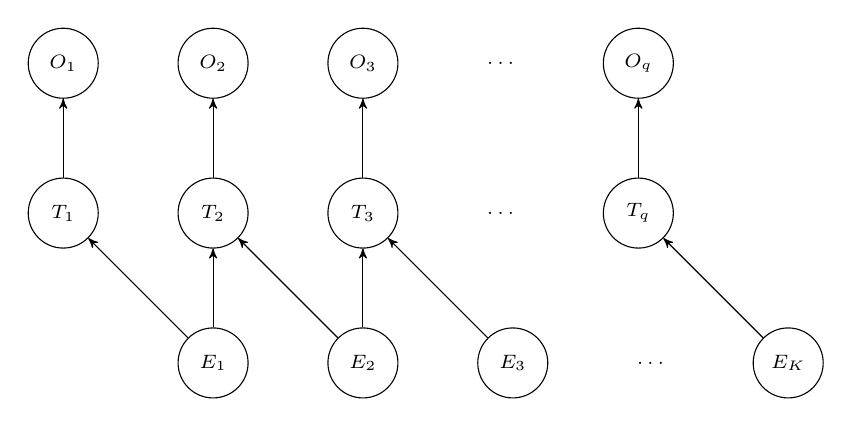
\begin{tikzpicture}[>=stealth',auto, font=\scriptsize]
  \tikzset{ellipse/.style={draw,ellipse}}

  \tikzset{
    blank/.style={
      text centered},
    circ/.style={
      circle,
      draw=black,
      minimum height=.35in,
      text centered}}

  \node[circ] (to1) {$O_1$};
  \node[circ] (to2) [right=of to1] {$O_2$};
  \node[circ] (to3) [right=of to2] {$O_3$};
  \node[blank] (tospace) [right=of to3] {$\ldots$};
  \node[circ] (ton) [right=of tospace] {$O_q$};

  \node[circ] (t1) [below=of to1] {$T_1$};
  \node[circ] (t2) [below=of to2] {$T_2$};
  \node[circ] (t3) [below=of to3] {$T_3$};
  \node[blank] (tspace) [right=of t3] {$\ldots$};
  \node[circ] (tn) [below=of ton] {$T_q$};

  \node[circ] (e1) [below=of t2] {$E_1$};
  \node[circ] (e2) [right=of e1] {$E_2$};
  \node[circ] (e3) [right=of e2] {$E_3$};
  \node[blank] (espace) [right=of e3] {$\ldots$};
  \node[circ] (ek) [right=of espace] {$E_K$};

  \path[->] (t1) edge (to1);
  \path[->] (t2) edge (to2);
  \path[->] (t3) edge (to3);
  \path[->] (tn) edge (ton);

  % Illustrative subset of E_k -> T_i edges
  \path[->] (e1) edge (t1);
  \path[->] (e1) edge (t2);

  \path[->] (e2) edge (t2);
  \path[->] (e2) edge (t3);

  \path[->] (e3) edge (t3);

  \path[->] (ek) edge (tn);

\end{tikzpicture}
\end{center}
\caption{Model for phenotypic effects of a variant with multiple endophenotypes}
\label{fig:variantbn_multiendo}
\end{figure}

We assume the $K$ endophenotype effects are independent \emph{a priori}
(and note that a full covariance prior could be substituted without
changing the inference strategy). We specify conditional probability
distributions as:
\[ E_k \sim {\mathcal N}\left(\mu_k, \tau_k^2\right) \qquad (k = 1,\ldots,K) \]
\[ T_i \sim {\mathcal N}\left(\sum_{k=1}^K \beta_{ik} E_k, \sigma_i^2\right) \qquad (i = 1,\ldots,q) \]
\[ O_i \sim {\mathcal N}\left(T_i, s_i^2\right) \qquad (i = 1,\ldots,q) \]

Here, $\beta_{ik}$ is the contribution of endophenotype $k$ to trait
$i$; equivalently, it is the strength of the edge $E_k \rightarrow
T_i$. In an implementation, the structure (which edges are permitted)
can be specified in a configuration file; if the edge $E_k \rightarrow
T_i$ is absent, we fix $\beta_{ik} = 0$.
As before, the $\sigma_i$ control how tightly trait $T_i$ follows the
endophenotype-driven profile, and $s_i$ controls the sampling
distribution of the observed association statistics. The parameters
$\mu_k$ and $\tau_k$ describe the prior population distribution of
endophenotype $k$.

For convenience, define the $q\times K$ matrix
$\mathbf{B} = \left(\beta_{ik}\right)$, the prior mean vector
$\mathbf{\mu} = \left(\mu_1,\ldots,\mu_K\right)^T$, and the prior
covariance
$\mathbf{\Sigma}_E = \mathrm{diag}\left(\tau_1^2,\ldots,\tau_K^2\right)$.
For each variant $j$, let
$\mathbf{o}^j = \left(o_1^j,\ldots,o_q^j\right)^T$ denote the observed
effects. Collapsing over $T_i$ as before yields
\[
O_i^j \mid \mathbf{E}^j \sim {\mathcal N}\left(\mathbf{b}_i^T\mathbf{E}^j,\ \sigma_i^2 + (s_i^j)^2\right),
\]
where $\mathbf{b}_i^T$ is the $i$th row of $\mathbf{B}$, and $s_i^j$ is
the (variant-specific) standard error for $O_i^j$.

Let $v_i^j = \sigma_i^2 + (s_i^j)^2$ and define the diagonal weight
matrix
\[
\mathbf{W}^j = \mathrm{diag}\left(\frac{1}{v_1^j},\ldots,\frac{1}{v_q^j}\right).
\]
Then the posterior distribution of $\mathbf{E}^j$ given the observations
$\mathbf{o}^j$ is multivariate normal:
\begin{eqnarray*}
\mathbf{E}^j \mid \mathbf{o}^j & \sim & {\mathcal N}\left(\mathbf{m}_E^j,\ \mathbf{V}_E^j\right) \\
\mathbf{V}_E^j & = & \left(\mathbf{\Sigma}_E^{-1} + \mathbf{B}^T \mathbf{W}^j \mathbf{B}\right)^{-1} \\
\mathbf{m}_E^j & = & \mathbf{V}_E^j\left(\mathbf{\Sigma}_E^{-1}\mathbf{\mu} + \mathbf{B}^T \mathbf{W}^j \mathbf{o}^j\right).
\end{eqnarray*}

For fitting the model using EM, the M-step requires expectations with
respect to the posterior. The basic sufficient statistics for variant
$j$ are
\[
\mathrm{E}\left[\mathbf{E}^j\right],\qquad
\mathrm{E}\left[\mathbf{E}^j\left(\mathbf{E}^j\right)^T\right],\qquad
\mathrm{E}\left[T_i^j \mathbf{E}^j\right],\qquad
\mathrm{E}\left[\left(T_i^j\right)^2\right].
\]
From the posterior above,
\[
\mathrm{E}\left[\mathbf{E}^j\right] = \mathbf{m}_E^j,
\qquad
\mathrm{E}\left[\mathbf{E}^j\left(\mathbf{E}^j\right)^T\right]
= \mathbf{V}_E^j + \mathbf{m}_E^j\left(\mathbf{m}_E^j\right)^T.
\]

Additionally, conditional on $\mathbf{E}^j$, the posterior of $T_i^j$
given $o_i^j$ remains univariate normal:
\begin{eqnarray*}
T_i^j \mid \mathbf{E}^j, o_i^j & \sim & {\mathcal N}\left(m_{T,i}^j(\mathbf{E}^j),\ V_{T,i}^j\right) \\
V_{T,i}^j & = & \left(\frac{1}{\sigma_i^2} + \frac{1}{(s_i^j)^2}\right)^{-1}
= \frac{\sigma_i^2 (s_i^j)^2}{\sigma_i^2 + (s_i^j)^2} \\
m_{T,i}^j(\mathbf{E}^j) & = & V_{T,i}^j\left(\frac{\mathbf{b}_i^T\mathbf{E}^j}{\sigma_i^2} + \frac{o_i^j}{(s_i^j)^2}\right).
\end{eqnarray*}
Define
\[
a_i^j = \frac{\sigma_i^2}{\sigma_i^2+(s_i^j)^2},\qquad
b_i^j = \frac{(s_i^j)^2}{\sigma_i^2+(s_i^j)^2}.
\]
Then $m_{T,i}^j(\mathbf{E}^j) = a_i^j o_i^j + b_i^j \mathbf{b}_i^T\mathbf{E}^j$.
Using the law of total expectation, we obtain
\begin{eqnarray*}
\mathrm{E}\left[T_i^j \mathbf{E}^j\right]
& = &
a_i^j o_i^j\,\mathbf{m}_E^j
+
b_i^j\left(\mathbf{V}_E^j + \mathbf{m}_E^j\left(\mathbf{m}_E^j\right)^T\right)\mathbf{b}_i \\
\mathrm{E}\left[\left(T_i^j\right)^2\right]
& = &
V_{T,i}^j
+
\left(a_i^j o_i^j\right)^2
+
2 a_i^j o_i^j b_i^j\, \mathbf{b}_i^T\mathbf{m}_E^j
+
\left(b_i^j\right)^2 \mathbf{b}_i^T
\left(\mathbf{V}_E^j + \mathbf{m}_E^j\left(\mathbf{m}_E^j\right)^T\right)\mathbf{b}_i.
\end{eqnarray*}

Differentiating the expected complete-data log-likelihood yields M-step
updates analogous to the single-endophenotype case. In particular, the
update for the $K$-vector of coefficients for trait $i$,
$\mathbf{b}_i$, is
\[
\mathbf{b}_i
=
\left(\sum_j \mathrm{E}\left[\mathbf{E}^j\left(\mathbf{E}^j\right)^T\right]\right)^{-1}
\left(\sum_j \mathrm{E}\left[T_i^j \mathbf{E}^j\right]\right),
\]
with the understanding that if the configuration fixes certain entries
of $\mathbf{b}_i$ to zero, the corresponding rows/columns should be
removed from the linear system and the fixed entries restored after
solving. The update for $\sigma_i^2$ is
\[
\sigma_i^2 = \frac{1}{N}\sum_j \mathrm{E}\left[\left(T_i^j - \mathbf{b}_i^T\mathbf{E}^j\right)^2\right],
\]
and the updates for $\mu_k$ and $\tau_k^2$ are
\[
\mu_k = \frac{1}{N}\sum_j \mathrm{E}\left[E_k^j\right],
\qquad
\tau_k^2 = \frac{1}{N}\sum_j \mathrm{E}\left[\left(E_k^j-\mu_k\right)^2\right].
\]

Finally, we note that inference can also be performed by Gibbs
sampling. In a Gibbs sampler, we alternate sampling
$T_i^j \mid \mathbf{E}^j,o_i^j$ using the univariate normal conditional
above, and sampling $\mathbf{E}^j \mid \mathbf{T}^j$ using the
multivariate normal conditional
\[
\mathbf{E}^j \mid \mathbf{T}^j \sim {\mathcal N}\left(\mathbf{m}_{E\mid T}^j,\ \mathbf{V}_{E\mid T}\right),
\]
where
\[
\mathbf{V}_{E\mid T} = \left(\mathbf{\Sigma}_E^{-1} + \mathbf{B}^T \mathrm{diag}\left(\frac{1}{\sigma_1^2},\ldots,\frac{1}{\sigma_q^2}\right)\mathbf{B}\right)^{-1},
\qquad
\mathbf{m}_{E\mid T}^j = \mathbf{V}_{E\mid T}\left(\mathbf{\Sigma}_E^{-1}\mathbf{\mu} + \mathbf{B}^T \mathrm{diag}\left(\frac{1}{\sigma_1^2},\ldots,\frac{1}{\sigma_q^2}\right)\mathbf{t}^j\right).
\]


\section{Extension to allow edges between traits}

We can extend the model to allow dependencies among traits not captured
by the endophenotypes by adding directed edges between the true trait
effects $T_1,\ldots,T_q$. Let $\mathrm{Pa}(i)$ denote the set of parent
traits of $T_i$ in a user-specified directed acyclic graph (DAG). For
each directed edge $T_p \rightarrow T_i$, introduce a coefficient
$\alpha_{ip}$ which captures the contribution of the true effect on
trait $p$ to the true effect on trait $i$, beyond what is explained by
the endophenotypes. If an edge $T_p \rightarrow T_i$ is absent from the
graph, we fix $\alpha_{ip} = 0$. The resulting graphical model is shown
in Figure \myref{fig:variantbn_traitdag}.

\begin{figure}[ht]
\begin{center}
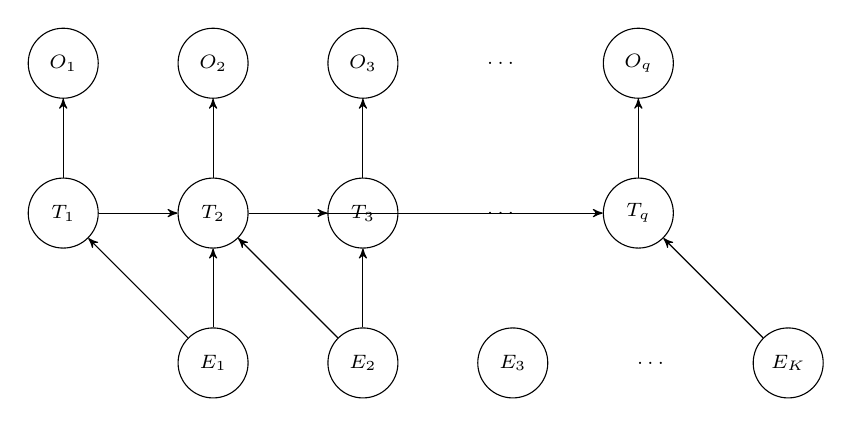
\begin{tikzpicture}[>=stealth',auto, font=\scriptsize]
  \tikzset{ellipse/.style={draw,ellipse}}

  \tikzset{
    blank/.style={
      text centered},
    circ/.style={
      circle,
      draw=black,
      minimum height=.35in,
      text centered}}

  \node[circ] (to1) {$O_1$};
  \node[circ] (to2) [right=of to1] {$O_2$};
  \node[circ] (to3) [right=of to2] {$O_3$};
  \node[blank] (tospace) [right=of to3] {$\ldots$};
  \node[circ] (ton) [right=of tospace] {$O_q$};

  \node[circ] (t1) [below=of to1] {$T_1$};
  \node[circ] (t2) [below=of to2] {$T_2$};
  \node[circ] (t3) [below=of to3] {$T_3$};
  \node[blank] (tspace) [right=of t3] {$\ldots$};
  \node[circ] (tn) [below=of ton] {$T_q$};

  \node[circ] (e1) [below=of t2] {$E_1$};
  \node[circ] (e2) [right=of e1] {$E_2$};
  \node[circ] (e3) [right=of e2] {$E_3$};
  \node[blank] (espace) [right=of e3] {$\ldots$};
  \node[circ] (ek) [right=of espace] {$E_K$};

  \path[->] (t1) edge (to1);
  \path[->] (t2) edge (to2);
  \path[->] (t3) edge (to3);
  \path[->] (tn) edge (ton);

  % Illustrative subset of E_k -> T_i edges
  \path[->] (e1) edge (t1);
  \path[->] (e1) edge (t2);
  \path[->] (e2) edge (t2);
  \path[->] (e2) edge (t3);
  \path[->] (ek) edge (tn);

  % Illustrative DAG edges between traits
  \path[->] (t1) edge (t2);
  \path[->] (t2) edge (t3);
  \path[->] (t2) edge (tn);

\end{tikzpicture}
\end{center}
\caption{Model for phenotypic effects of a variant with multiple endophenotypes and directed edges between traits}
\label{fig:variantbn_traitdag}
\end{figure}

We then specify
\[
T_i \sim {\mathcal N}\left(\mathbf{b}_i^T\mathbf{E} + \sum_{p\in\mathrm{Pa}(i)} \alpha_{ip} T_p,\ \sigma_i^2\right),
\qquad
O_i \sim {\mathcal N}\left(T_i,\ s_i^2\right),
\]
together with the prior on $\mathbf{E}$ from the previous section.
Because the trait graph is required to be a DAG, there exists a
topological ordering of traits under which each trait depends only on
traits earlier in the ordering; if a cycle is present, the model does
not define a valid Bayesian network and inference should be refused.

It is convenient to write this extension in matrix form. Let
$\mathbf{A}$ be the $q\times q$ matrix with entries
$(\mathbf{A})_{ip} = \alpha_{ip}$, and define
$\mathbf{L} = \mathbf{I} - \mathbf{A}$. Under the DAG assumption,
$\mathbf{L}$ is invertible. Let
$\mathbf{D} = \mathrm{diag}\left(\sigma_1^2,\ldots,\sigma_q^2\right)$.
Then the trait model can be written as the linear structural equation
\[
\mathbf{L}\mathbf{T}^j = \mathbf{B}\mathbf{E}^j + \boldsymbol{\varepsilon}^j,
\qquad
\boldsymbol{\varepsilon}^j \sim {\mathcal N}\left(\mathbf{0},\mathbf{D}\right),
\]
and hence
\begin{eqnarray*}
\mathbf{T}^j \mid \mathbf{E}^j & \sim & {\mathcal N}\left(\mathbf{M}\mathbf{E}^j,\ \mathbf{\Sigma}_T\right) \\
\mathbf{M} & = & \mathbf{L}^{-1}\mathbf{B} \\
\mathbf{\Sigma}_T & = & \mathbf{L}^{-1}\mathbf{D}\left(\mathbf{L}^{-1}\right)^T.
\end{eqnarray*}

The observation model remains conditionally independent given
$\mathbf{T}^j$. Let
$\mathbf{S}^j = \mathrm{diag}\left((s_1^j)^2,\ldots,(s_q^j)^2\right)$.
Then, collapsing over $\mathbf{T}^j$ yields
\[
\mathbf{O}^j \mid \mathbf{E}^j \sim {\mathcal N}\left(\mathbf{M}\mathbf{E}^j,\ \mathbf{V}^j\right),
\qquad
\mathbf{V}^j = \mathbf{\Sigma}_T + \mathbf{S}^j.
\]
As above, the posterior distribution of $\mathbf{E}^j$ given
$\mathbf{o}^j$ is multivariate normal:
\begin{eqnarray*}
\mathbf{E}^j \mid \mathbf{o}^j & \sim & {\mathcal N}\left(\mathbf{m}_E^j,\ \mathbf{V}_E^j\right) \\
\mathbf{V}_E^j & = & \left(\mathbf{\Sigma}_E^{-1} + \mathbf{M}^T\left(\mathbf{V}^j\right)^{-1}\mathbf{M}\right)^{-1} \\
\mathbf{m}_E^j & = & \mathbf{V}_E^j\left(\mathbf{\Sigma}_E^{-1}\mathbf{\mu} + \mathbf{M}^T\left(\mathbf{V}^j\right)^{-1}\mathbf{o}^j\right).
\end{eqnarray*}

In addition, the posterior mean of the true trait effects can be
computed in closed form. Since
$\mathbf{T}^j\mid\mathbf{E}^j$ and $\mathbf{O}^j\mid\mathbf{T}^j$ are
both multivariate normal, we have
\[
\mathrm{E}\left[\mathbf{T}^j \mid \mathbf{o}^j\right]
=
\mathbf{M}\mathbf{m}_E^j
+
\mathbf{\Sigma}_T\left(\mathbf{V}^j\right)^{-1}\left(\mathbf{o}^j - \mathbf{M}\mathbf{m}_E^j\right).
\]
For fitting the model using EM, the sufficient statistics can be
obtained from the joint multivariate normal posterior of
$(\mathbf{E}^j,\mathbf{T}^j)\mid \mathbf{o}^j$, and the M-step updates
for $(\mathbf{b}_i,\{\alpha_{ip}\}_{p\in\mathrm{Pa}(i)})$ correspond to
a linear regression of $T_i$ on the predictors
$\left(\mathbf{E},\mathbf{T}_{\mathrm{Pa}(i)}\right)$ using posterior
expected cross-products.

As in the previous section, inference can also be performed by Gibbs
sampling. One convenient Gibbs scheme alternates the block updates
\[
\mathbf{T}^j \mid \mathbf{E}^j,\mathbf{o}^j \sim {\mathcal N}\left(\mathbf{m}_{T\mid E}^j,\ \mathbf{\Sigma}_{T\mid E}^j\right),
\qquad
\mathbf{E}^j \mid \mathbf{T}^j \sim {\mathcal N}\left(\mathbf{m}_{E\mid T}^j,\ \mathbf{V}_{E\mid T}\right),
\]
where
\begin{eqnarray*}
\mathbf{m}_{T\mid E}^j & = & \mathbf{M}\mathbf{E}^j + \mathbf{\Sigma}_T\left(\mathbf{V}^j\right)^{-1}\left(\mathbf{o}^j - \mathbf{M}\mathbf{E}^j\right) \\
\mathbf{\Sigma}_{T\mid E}^j & = & \mathbf{\Sigma}_T - \mathbf{\Sigma}_T\left(\mathbf{V}^j\right)^{-1}\mathbf{\Sigma}_T.
\end{eqnarray*}
For the $\mathbf{E}^j \mid \mathbf{T}^j$ update, define
$\mathbf{y}^j = \mathbf{L}\mathbf{T}^j$. Then
$\mathbf{y}^j \mid \mathbf{E}^j \sim {\mathcal N}\left(\mathbf{B}\mathbf{E}^j,\mathbf{D}\right)$, and hence
\begin{eqnarray*}
\mathbf{V}_{E\mid T} & = & \left(\mathbf{\Sigma}_E^{-1} + \mathbf{B}^T \mathbf{D}^{-1}\mathbf{B}\right)^{-1} \\
\mathbf{m}_{E\mid T}^j & = & \mathbf{V}_{E\mid T}\left(\mathbf{\Sigma}_E^{-1}\mathbf{\mu} + \mathbf{B}^T \mathbf{D}^{-1}\mathbf{y}^j\right).
\end{eqnarray*}
Alternatively, one can update the trait nodes $T_i$ one-at-a-time using
their Markov blanket in the trait DAG; the resulting full conditionals
are univariate normal.

\section{Control for outlier traits}

A practical failure mode of the base model is that a single trait with an
extremely strong observed association can force the posterior endophenotype
$\mathbf{E}^j$ to be large, because the model has no other mechanism to explain
a highly unlikely observation. In applications where we seek variants that
match a coherent multi-trait pattern (rather than variants driven by a single
trait), this behavior is undesirable.

We address this by introducing, for each trait $i$ and variant $j$, a binary
indicator $Z_i^j \in \{0,1\}$ which controls an inflation of the residual
variance in the trait layer. Intuitively, when $Z_i^j = 1$ trait $i$ is treated
as an ``outlier'' for variant $j$ and is given less influence on the inferred
endophenotypes.

\subsection*{Model definition}

Let $\kappa > 1$ denote a variance inflation factor. Let $\pi_i \in (0,1)$ be
the prior probability that trait $i$ is an outlier for a randomly chosen
variant. (In many applications we will impose $\pi_i \equiv \pi$ for all traits
for stability and interpretability.)

For each variant $j$ and trait $i$, define
\[
Z_i^j \sim \mathrm{Bernoulli}(\pi_i),
\qquad
c(Z_i^j) =
\begin{cases}
1, & Z_i^j = 0 \\
\kappa^2, & Z_i^j = 1.
\end{cases}
\]
We extend the trait layer to
\[
T_i^j \mid \mathbf{E}^j,\mathbf{T}_{\mathrm{Pa}(i)}^j,Z_i^j
\sim
{\mathcal N}\left(\mathbf{b}_i^T\mathbf{E}^j + \sum_{p\in\mathrm{Pa}(i)}\alpha_{ip}T_p^j,\ \sigma_i^2\,c(Z_i^j)\right),
\]
and retain the observation model
\[
O_i^j \mid T_i^j \sim {\mathcal N}\left(T_i^j,\ (s_i^j)^2\right).
\]
When $Z_i^j = 1$, the increased variance $\kappa^2\sigma_i^2$ reduces the
leverage of trait $i$ on $\mathbf{E}^j$ and on the fitted loadings, providing a
mechanism to ``soak up'' trait-specific signals that do not align with the
multi-trait pattern.

It is convenient to write this in matrix form (as in the trait-edge extension).
Let $\mathbf{A}$ be the matrix of trait-edge coefficients, and let
$\mathbf{L} = \mathbf{I} - \mathbf{A}$. For each variant $j$, define the
diagonal matrix
\[
\mathbf{D}^j(\mathbf{Z}^j) = \mathrm{diag}\left(\sigma_1^2 c(Z_1^j),\ldots,\sigma_q^2 c(Z_q^j)\right).
\]
Conditional on $\mathbf{Z}^j = (Z_1^j,\ldots,Z_q^j)$, the trait layer becomes
\[
\mathbf{L}\mathbf{T}^j = \mathbf{B}\mathbf{E}^j + \boldsymbol{\varepsilon}^j,
\qquad
\boldsymbol{\varepsilon}^j \sim {\mathcal N}\left(\mathbf{0},\mathbf{D}^j(\mathbf{Z}^j)\right).
\]
Therefore
\begin{eqnarray*}
\mathbf{T}^j \mid \mathbf{E}^j,\mathbf{Z}^j & \sim &
{\mathcal N}\left(\mathbf{M}\mathbf{E}^j,\ \mathbf{\Sigma}_T^j(\mathbf{Z}^j)\right) \\
\mathbf{M} & = & \mathbf{L}^{-1}\mathbf{B} \\
\mathbf{\Sigma}_T^j(\mathbf{Z}^j) & = &
\mathbf{L}^{-1}\mathbf{D}^j(\mathbf{Z}^j)\left(\mathbf{L}^{-1}\right)^T.
\end{eqnarray*}
Let $\mathbf{S}^j = \mathrm{diag}\left((s_1^j)^2,\ldots,(s_q^j)^2\right)$.
Collapsing over $\mathbf{T}^j$ yields
\[
\mathbf{O}^j \mid \mathbf{E}^j,\mathbf{Z}^j \sim
{\mathcal N}\left(\mathbf{M}\mathbf{E}^j,\ \mathbf{V}^j(\mathbf{Z}^j)\right),
\qquad
\mathbf{V}^j(\mathbf{Z}^j) = \mathbf{\Sigma}_T^j(\mathbf{Z}^j) + \mathbf{S}^j.
\]

\begin{figure}[ht]
\begin{center}
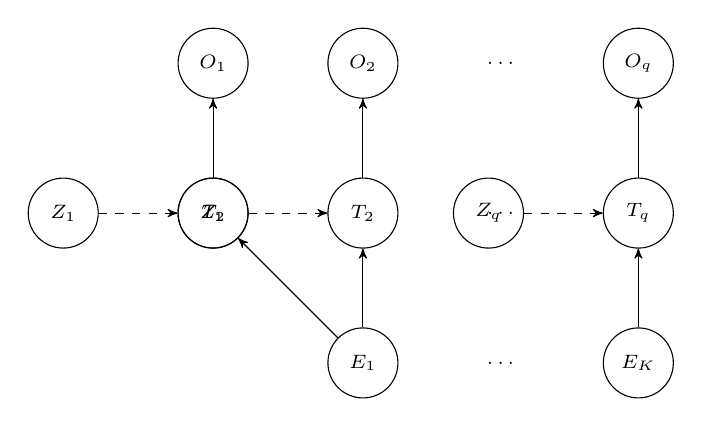
\begin{tikzpicture}[>=stealth',auto, font=\scriptsize]
  \tikzset{
    blank/.style={text centered},
    circ/.style={circle, draw=black, minimum height=.35in, text centered}
  }

  \node[circ] (to1) {$O_1$};
  \node[circ] (to2) [right=of to1] {$O_2$};
  \node[blank] (tospace) [right=of to2] {$\ldots$};
  \node[circ] (ton) [right=of tospace] {$O_q$};

  \node[circ] (t1) [below=of to1] {$T_1$};
  \node[circ] (t2) [below=of to2] {$T_2$};
  \node[blank] (tspace) [right=of t2] {$\ldots$};
  \node[circ] (tn) [below=of ton] {$T_q$};

  \node[circ] (z1) [left=of t1] {$Z_1$};
  \node[circ] (z2) [left=of t2] {$Z_2$};
  \node[circ] (zn) [left=of tn] {$Z_q$};

  \node[circ] (e1) [below=of t2] {$E_1$};
  \node[blank] (espace) [right=of e1] {$\ldots$};
  \node[circ] (ek) [right=of espace] {$E_K$};

  \path[->] (t1) edge (to1);
  \path[->] (t2) edge (to2);
  \path[->] (tn) edge (ton);

  \path[->] (e1) edge (t1);
  \path[->] (e1) edge (t2);
  \path[->] (ek) edge (tn);

  \path[dashed,->] (z1) edge (t1);
  \path[dashed,->] (z2) edge (t2);
  \path[dashed,->] (zn) edge (tn);

\end{tikzpicture}
\end{center}
\caption{Adding per-trait outlier indicators $Z_i$ that inflate the residual variance in the trait layer by a factor $\kappa^2$ when $Z_i=1$}
\label{fig:variantbn_outliers}
\end{figure}

\subsection*{Estimation: analytic (exact) E-step by enumerating $\mathbf{Z}^j$}

Conditional on $\mathbf{Z}^j$, the model remains linear-Gaussian, so the
posterior of $\mathbf{E}^j$ given $\mathbf{o}^j$ and $\mathbf{Z}^j$ is
multivariate normal:
\begin{eqnarray*}
\mathbf{E}^j \mid \mathbf{o}^j,\mathbf{Z}^j
& \sim & {\mathcal N}\left(\mathbf{m}_E^j(\mathbf{Z}^j),\ \mathbf{V}_E^j(\mathbf{Z}^j)\right) \\
\mathbf{V}_E^j(\mathbf{Z}^j)
& = &
\left(\mathbf{\Sigma}_E^{-1} + \mathbf{M}^T\left(\mathbf{V}^j(\mathbf{Z}^j)\right)^{-1}\mathbf{M}\right)^{-1} \\
\mathbf{m}_E^j(\mathbf{Z}^j)
& = &
\mathbf{V}_E^j(\mathbf{Z}^j)\left(\mathbf{\Sigma}_E^{-1}\mathbf{\mu}
+ \mathbf{M}^T\left(\mathbf{V}^j(\mathbf{Z}^j)\right)^{-1}\mathbf{o}^j\right).
\end{eqnarray*}
Similarly, the posterior mean of $\mathbf{T}^j$ conditional on $\mathbf{Z}^j$
is
\[
\mathrm{E}\left[\mathbf{T}^j \mid \mathbf{o}^j,\mathbf{Z}^j\right]
=
\mathbf{M}\mathbf{m}_E^j(\mathbf{Z}^j)
+
\mathbf{\Sigma}_T^j(\mathbf{Z}^j)\left(\mathbf{V}^j(\mathbf{Z}^j)\right)^{-1}
\left(\mathbf{o}^j - \mathbf{M}\mathbf{m}_E^j(\mathbf{Z}^j)\right).
\]

To obtain the unconditional posterior, we marginalize over
$\mathbf{Z}^j \in \{0,1\}^q$:
\[
\Pr(\mathbf{Z}^j=\mathbf{z}) = \prod_{i=1}^q \pi_i^{z_i}(1-\pi_i)^{1-z_i},
\qquad
\Pr(\mathbf{Z}^j=\mathbf{z}\mid \mathbf{o}^j)
\propto
\Pr(\mathbf{Z}^j=\mathbf{z})\,\Pr(\mathbf{o}^j\mid \mathbf{Z}^j=\mathbf{z}).
\]
Since $\mathbf{o}^j\mid \mathbf{Z}^j$ is Gaussian after integrating out
$\mathbf{E}^j$, $\Pr(\mathbf{o}^j\mid \mathbf{Z}^j=\mathbf{z})$ can be computed
in closed form, and the posterior over $\mathbf{Z}^j$ can be normalized by
summing over all $2^q$ configurations.

Let $\gamma^j(\mathbf{z}) = \Pr(\mathbf{Z}^j=\mathbf{z}\mid \mathbf{o}^j)$.
Then posterior expectations are mixture averages, for example
\[
\mathrm{E}\left[\mathbf{E}^j\mid \mathbf{o}^j\right]
=
\sum_{\mathbf{z}} \gamma^j(\mathbf{z})\,\mathbf{m}_E^j(\mathbf{z}),
\qquad
\mathrm{E}\left[\mathbf{E}^j(\mathbf{E}^j)^T\mid \mathbf{o}^j\right]
=
\sum_{\mathbf{z}} \gamma^j(\mathbf{z})
\left(\mathbf{V}_E^j(\mathbf{z}) + \mathbf{m}_E^j(\mathbf{z})\mathbf{m}_E^j(\mathbf{z})^T\right).
\]
The outlier responsibility for trait $i$ at variant $j$ is
\[
\phi_i^j \equiv \Pr(Z_i^j=1\mid \mathbf{o}^j)
=
\sum_{\mathbf{z}} \gamma^j(\mathbf{z})\,z_i.
\]

For EM training with fixed $(\kappa,\pi_i)$, the M-step updates for the trait
coefficients become weighted least squares. Define the regression residual
\[
r_i^j = T_i^j - \mathbf{b}_i^T\mathbf{E}^j - \sum_{p\in\mathrm{Pa}(i)} \alpha_{ip}T_p^j.
\]
Then, using the expected complete-data log-likelihood, the variance update is
\[
\sigma_i^2
=
\frac{1}{\sum_j w_j}
\sum_j w_j\,\mathrm{E}\left[\frac{\left(r_i^j\right)^2}{c(Z_i^j)}\ \Big|\ \mathbf{\hat{O}}\right],
\]
and the coefficient updates for $(\mathbf{b}_i,\{\alpha_{ip}\})$ correspond to
solving the normal equations formed from the weighted cross-products
$\mathrm{E}\left[\left(\mathbf{E}^j,\mathbf{T}_{\mathrm{Pa}(i)}^j\right)
\left(\mathbf{E}^j,\mathbf{T}_{\mathrm{Pa}(i)}^j\right)^T/c(Z_i^j)\right]$ and
$\mathrm{E}\left[T_i^j\left(\mathbf{E}^j,\mathbf{T}_{\mathrm{Pa}(i)}^j\right)^T/c(Z_i^j)\right]$.

This analytic approach is exact, but its cost grows as $O(2^q)$ per variant and
is only practical for small numbers of traits.

\subsection*{Estimation: variational approximation}

For larger $q$, we can approximate the posterior with a mean-field family
\[
q(\mathbf{E}^j,\mathbf{T}^j,\mathbf{Z}^j)
=
q(\mathbf{E}^j,\mathbf{T}^j)\prod_{i=1}^q q(Z_i^j),
\qquad
q(Z_i^j=1)=\phi_i^j.
\]
Define
\[
\alpha_i^j \equiv \mathrm{E}_q\left[\frac{1}{c(Z_i^j)}\right]
=
(1-\phi_i^j) + \frac{\phi_i^j}{\kappa^2}.
\]
A standard coordinate ascent update yields $q(\mathbf{E}^j,\mathbf{T}^j)$ as a
Gaussian distribution obtained by replacing the diagonal residual covariance
$\mathbf{D}^j(\mathbf{Z}^j)$ with an effective covariance
\[
\widetilde{\mathbf{D}}^j \equiv \mathrm{diag}\left(\frac{\sigma_1^2}{\alpha_1^j},\ldots,\frac{\sigma_q^2}{\alpha_q^j}\right),
\qquad
\widetilde{\mathbf{\Sigma}}_T^j
=
\mathbf{L}^{-1}\widetilde{\mathbf{D}}^j\left(\mathbf{L}^{-1}\right)^T,
\qquad
\widetilde{\mathbf{V}}^j
=
\widetilde{\mathbf{\Sigma}}_T^j + \mathbf{S}^j.
\]
Thus the approximate posterior of $\mathbf{E}^j$ is
\begin{eqnarray*}
q(\mathbf{E}^j) & = & {\mathcal N}\left(\widetilde{\mathbf{m}}_E^j,\ \widetilde{\mathbf{V}}_E^j\right) \\
\widetilde{\mathbf{V}}_E^j
& = &
\left(\mathbf{\Sigma}_E^{-1} + \mathbf{M}^T\left(\widetilde{\mathbf{V}}^j\right)^{-1}\mathbf{M}\right)^{-1} \\
\widetilde{\mathbf{m}}_E^j
& = &
\widetilde{\mathbf{V}}_E^j\left(\mathbf{\Sigma}_E^{-1}\mathbf{\mu}
+ \mathbf{M}^T\left(\widetilde{\mathbf{V}}^j\right)^{-1}\mathbf{o}^j\right).
\end{eqnarray*}

The Bernoulli factors update via the log-odds
\[
\log\frac{\phi_i^j}{1-\phi_i^j}
=
\log\frac{\pi_i}{1-\pi_i}
-
\frac{1}{2}\log\kappa^2
+
\frac{1}{2}\left(1-\frac{1}{\kappa^2}\right)
\frac{\mathrm{E}_q\left[\left(\epsilon_i^j\right)^2\right]}{\sigma_i^2},
\]
where $\boldsymbol{\epsilon}^j = \mathbf{L}\mathbf{T}^j - \mathbf{B}\mathbf{E}^j$.
Because $\boldsymbol{\epsilon}^j$ is linear in $(\mathbf{T}^j,\mathbf{E}^j)$ and
$q(\mathbf{T}^j,\mathbf{E}^j)$ is Gaussian, the moment
$\mathrm{E}_q[(\epsilon_i^j)^2]$ can be computed from the posterior mean and
covariance. Iterating these updates yields a scalable approximation which avoids
the $2^q$ enumeration, at the cost of a mean-field approximation that typically
underestimates posterior uncertainty.

For EM training, the M-step uses the same weighted least squares form as above,
with the replacement $\mathrm{E}[1/c(Z_i^j)] \approx \alpha_i^j$ and
$\mathrm{E}[(r_i^j)^2/c(Z_i^j)] \approx \alpha_i^j\,\mathrm{E}_q[(r_i^j)^2]$.

\subsection*{Estimation: Gibbs sampling}

Finally, we can sample from the posterior by extending the existing Gibbs
sampler with updates for $\mathbf{Z}^j$.

Given $(\mathbf{E}^j,\mathbf{T}^j)$, each $Z_i^j$ is conditionally independent
with
\[
\Pr(Z_i^j=1\mid \mathbf{E}^j,\mathbf{T}^j,\mathbf{o}^j)
=
\frac{\pi_i\,{\mathcal N}(\epsilon_i^j;0,\kappa^2\sigma_i^2)}
{\pi_i\,{\mathcal N}(\epsilon_i^j;0,\kappa^2\sigma_i^2) + (1-\pi_i)\,{\mathcal N}(\epsilon_i^j;0,\sigma_i^2)},
\]
where $\boldsymbol{\epsilon}^j = \mathbf{L}\mathbf{T}^j - \mathbf{B}\mathbf{E}^j$.
Thus $Z_i^j$ can be drawn by a Bernoulli step using the above probability.

Conditional on $\mathbf{Z}^j$, the updates for $\mathbf{E}^j$ and $\mathbf{T}^j$
remain Gaussian. For example,
\[
\mathbf{E}^j \mid \mathbf{T}^j,\mathbf{Z}^j \sim
{\mathcal N}\left(\mathbf{m}_{E\mid T}^j,\ \mathbf{V}_{E\mid T}^j\right),
\qquad
\mathbf{V}_{E\mid T}^j =
\left(\mathbf{\Sigma}_E^{-1} + \mathbf{B}^T\left(\mathbf{D}^j(\mathbf{Z}^j)\right)^{-1}\mathbf{B}\right)^{-1},
\]
and $\mathbf{m}_{E\mid T}^j$ follows by conjugacy using $\mathbf{L}\mathbf{T}^j$
as the Gaussian observation for $\mathbf{B}\mathbf{E}^j$.

The conditional for each $T_i^j$ can be updated as in the trait-edge Gibbs
scheme, except that each occurrence of $\sigma_i^2$ is replaced by
$\sigma_i^2 c(Z_i^j)$, and child contributions use the corresponding child
variance $\sigma_c^2 c(Z_c^j)$.

Gibbs sampling is asymptotically exact and can handle large numbers of traits
and complex trait graphs, but it can be slower and requires burn-in and
convergence diagnostics. In contrast, analytic enumeration is exact but only
feasible for small $q$, and the variational approximation is scalable and fast
but approximate. When $q$ is small, the analytic approach dominates. For moderate
or large $q$ without requiring exact posterior uncertainty, the variational
approximation is usually preferred. Gibbs sampling is most appropriate when
exactness is important or when the variational approximation is unstable, at
the cost of runtime.

\section{Determining $\kappa$ and $\pi$}

The hyperparameters $\kappa$ and $\pi_i$ control how aggressively the model
downweights trait-specific outliers. These parameters are not reliably
identified from positives alone, and in many applications we choose them to
optimize separation between a curated positive set and a large background set of
variants. We therefore recommend selecting $(\kappa,\pi)$ by cross-validation
with an objective that emphasizes the extreme tail of the ranked list, which is
the relevant regime for genome-wide screening.

\subsection*{Scoring function}

For each variant $j$, inference under a fixed $(\kappa,\pi)$ yields a posterior
mean and covariance for $\mathbf{E}^j$, denoted $(\mathbf{m}_E^j,\mathbf{V}_E^j)$
(using analytic, variational, or Gibbs inference). We define an endophenotype
evidence score
\[
S^j \equiv \left(\mathbf{m}_E^j\right)^T\left(\mathbf{V}_E^j\right)^{-1}\mathbf{m}_E^j,
\]
which is the squared Mahalanobis norm of the posterior mean. In the
single-endophenotype case this reduces to the squared posterior $z$-score
$(m_E^j / \sqrt{V_E^j})^2$. This score increases when the data support a coherent
endophenotype signal with small posterior uncertainty, and it decreases when the
signal is explained instead by one or more outlier indicators $Z_i^j$.

\subsection*{Composite cross-validation metric}

Let $\mathcal{P}$ denote the curated positive set. Let $\mathcal{B}$ denote a
large background set (e.g., random variants from the genome-wide set excluding
$\mathcal{P}$). Optionally, let $\mathcal{H}$ denote a ``hard negative'' set
(e.g., variants significant for one trait but not others).

For a target background false positive rate $\alpha$ (e.g., $\alpha=10^{-3}$ or
$10^{-4}$), define the threshold $t_\alpha$ as the $(1-\alpha)$ empirical
quantile of $S^j$ over $\mathcal{B}$. Define
\[
\mathrm{TPR}_\alpha = \frac{1}{|\mathcal{P}|}\sum_{j\in\mathcal{P}} \mathbf{1}\{S^j \ge t_\alpha\},
\qquad
\mathrm{FPR}_{\alpha,\mathrm{hard}} = \frac{1}{|\mathcal{H}|}\sum_{j\in\mathcal{H}} \mathbf{1}\{S^j \ge t_\alpha\}.
\]
We propose the composite metric
\[
\mathrm{Score}(\kappa,\pi)
=
\frac{1}{|\mathcal{A}|}\sum_{\alpha\in\mathcal{A}}
\left(\mathrm{TPR}_\alpha - \lambda\,\mathrm{FPR}_{\alpha,\mathrm{hard}}\right),
\]
where $\mathcal{A}$ is a small set of tail operating points (e.g.,
$\{10^{-3},10^{-4}\}$) and $\lambda \ge 0$ is a penalty weight (e.g.,
$\lambda=1$). If no hard-negative set is available, we set $\lambda=0$.

This metric directly targets performance in the extreme tail while guarding
against trivial improvements that simply inflate scores for many single-trait
signals.

\subsection*{Cross-validation procedure}

We recommend selecting $(\kappa,\pi)$ over a grid (typically log-spaced for $\pi$
and a small set of $\kappa$ values). Let $\mathcal{P}$ be split into $K$ folds
$\mathcal{P}_1,\ldots,\mathcal{P}_K$. For each grid point $(\kappa,\pi)$, we
repeat:

\begin{enumerate}
\item For each fold $k$:
  \begin{enumerate}
  \item Train model parameters $\theta$ on $\mathcal{P}\setminus\mathcal{P}_k$
        using EM (with the chosen inference method) holding $(\kappa,\pi)$ fixed.
  \item Compute scores $S^j$ for $j\in\mathcal{P}_k$, and for sampled sets from
        $\mathcal{B}$ (and $\mathcal{H}$, if used).
  \item Compute the composite metric for fold $k$.
  \end{enumerate}
\item Average the fold metrics to obtain $\mathrm{Score}(\kappa,\pi)$.
\end{enumerate}
Select the grid point with the largest score, then retrain $\theta$ on the full
positive set $\mathcal{P}$ using the selected $(\kappa,\pi)$.

\subsection*{Fast abbreviated option}

The procedure above is statistically clean but can be expensive because EM is
nested inside the cross-validation loop. A faster approximation is:

\begin{enumerate}
\item Train $\theta$ once on all positives using a reasonable default
      $(\kappa,\pi)$ (or with $\pi=0$ as a baseline).
\item Holding $\theta$ fixed, choose $(\kappa,\pi)$ by cross-validation using
      only the inference step and the scoring metric above.
\item Optionally run a final EM training pass using the selected $(\kappa,\pi)$.
\end{enumerate}

This abbreviated procedure is appropriate when the fitted structural parameters
$\theta$ are relatively stable across plausible choices of $(\kappa,\pi)$, which
is often the case when $\kappa$ and $\pi$ primarily modulate how outliers are
downweighted rather than changing the coherent multi-trait signal.

Because the prior outlier probability $\pi$ depends on the number of traits $q$, it is often more
interpretable to parameterize the outlier rate in terms of the expected number of outlier traits per
variant. Define
\[
\lambda_{\mathrm{out}} \equiv \mathrm{E}\left[\sum_{i=1}^q Z_i^j\right] = \sum_{i=1}^q \pi_i.
\]
In the common case of a shared outlier probability $\pi_i \equiv \pi$ for all traits, this reduces to
$\lambda_{\mathrm{out}} = q\pi$ and hence $\pi = \lambda_{\mathrm{out}}/q$. This reparameterization makes
hyperparameter choices stable as $q$ changes (e.g., when moving from $q\approx 10$ traits to
$q\approx 50$ traits), since fixing $\lambda_{\mathrm{out}}$ fixes the prior expected number of outlier
traits rather than implicitly allowing more outliers as additional traits are added. In practice, we
therefore tune over a grid of $(\kappa,\lambda_{\mathrm{out}})$ and convert to $\pi=\lambda_{\mathrm{out}}/q$
within each run. When the cross-validation objective is relatively flat across a range of values, we
recommend a conservative tie-breaking rule analogous to the one-standard-error rule: among all
grid points whose mean cross-validation score is within one estimated standard error of the best
mean score, select the point with the smallest $\lambda_{\mathrm{out}}$ (fewest expected outlier traits)
and, if tied, the smallest $\kappa$ (least aggressive variance inflation).


\end{document}


